\chapter{Eenheden, dimensies en meten}\label{ch:b1:units-dimensions}

In een kelderlaboratorium zwaait een slinger, klikt een stopwatch en
schrijft een student $g = \qty{9.77}{m/s^2}$ op. Is dat de ``juiste''
waarde? Het handboek zegt $9.81$. Of die twee getallen overeenstemmen, of
de proef goed was opgezet, welke stap haar begrensde --- niets daarvan valt
uit de cijfers alleen op te maken. Natuurkunde meet, en een meting zonder
haar onzekerheid is een gerucht. Dit hoofdstuk legt de gemeenschappelijke
taal van alle volgende hoofdstukken vast: eenheden, \omterm{def:b1:units-dimensions:dimension}{dimensies}, ordes van
grootte en het eerlijke rekenwerk met onzekerheden.

\begin{omfigure}
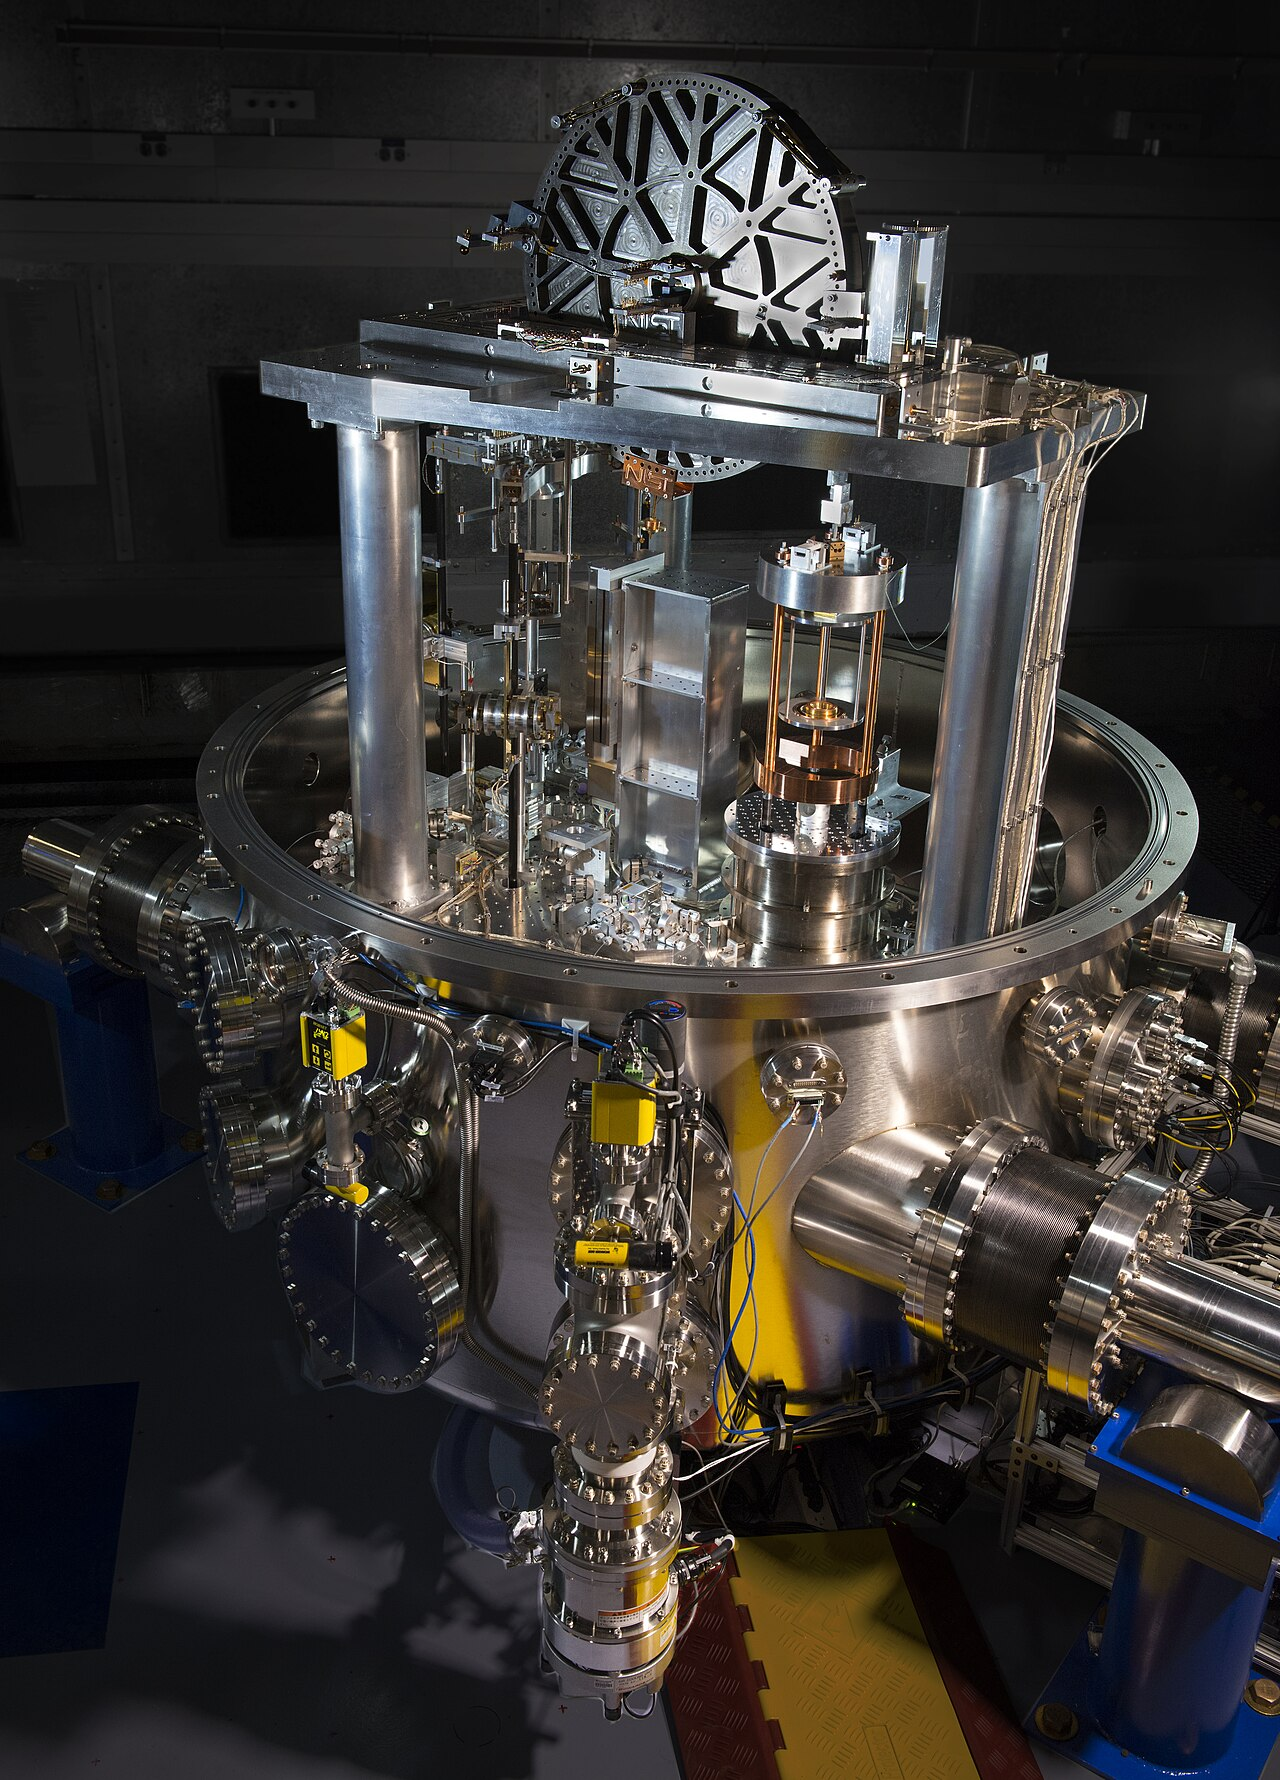
\includegraphics[width=0.46\linewidth]{images/book3/kibble-balance-nist.jpg}

{\small De Kibble-balans NIST-4, een van de instrumenten die de kilogram nu uit de constante van Planck realiseren: een massa wordt afgewogen tegen een elektromagnetische kracht die in elektrische eenheden wordt gemeten. Foto: J.~L.~Lee, NIST (publiek domein).}
\end{omfigure}

\section{Het Internationale Stelsel van Eenheden}

\begin{definition}[Grootheid en eenheid]\label{def:b1:units-dimensions:unit}
Een \emph{natuurkundige grootheid}\index{natuurkundige grootheid} is een
eigenschap die gemeten kan worden: een lengte, een tijdsduur, een massa,
een stroom. Haar meten betekent haar vergelijken met een referentie van
dezelfde soort, de \emph{eenheid}\index{eenheid}: het resultaat is een
getal maal een eenheid, $\ell = \qty{1.257}{m}$. Het getal alleen betekent
niets; de eenheid alleen meet niets.
\end{definition}

\begin{definition}[Basiseenheden van het SI]\label{def:b1:units-dimensions:si}
\index{SI (Internationaal Stelsel van Eenheden)}\index{basiseenheid}
Het \emph{Internationale Stelsel van Eenheden} (SI) berust op zeven
\emph{basiseenheden}: de seconde (\unit{s}), de meter (\unit{m}), de
kilogram (\unit{kg}), de ampère (\unit{A}), de kelvin (\unit{K}), de
mol (\unit{mol}) en de candela (\unit{cd}). Sinds 2019 wordt elk daarvan
vastgelegd door de getalwaarde van een natuurconstante vast te leggen: de
hyperfijnovergang van cesium $\Delta\nu_{\mathrm{Cs}} = \qty{9192631770}{Hz}$
legt de seconde vast; de lichtsnelheid $c = \qty{299792458}{m/s}$ legt
vervolgens de meter vast; de constante van Planck
$h = \qty{6.62607015e-34}{J.s}$ de kilogram; de elementaire
lading $e = \qty{1.602176634e-19}{C}$ de ampère; de constante van Boltzmann
$k_B = \qty{1.380649e-23}{J/K}$ de kelvin; de constante van Avogadro
$N_A = \qty{6.02214076e23}{mol^{-1}}$ de mol; en een vaste lichtstroom
per watt $K_{\mathrm{cd}}$ de candela. Elke andere \omterm{def:b1:units-dimensions:unit}{eenheid} is een
\emph{afgeleide eenheid}\index{afgeleide eenheid}, een product van machten
van basiseenheden: $\qty{1}{N} = \qty{1}{kg.m/s^2}$, $\qty{1}{J} = \qty{1}{N.m}$,
$\qty{1}{W} = \qty{1}{J/s}$, $\qty{1}{V} = \qty{1}{W/A}$,
$\qty{1}{Pa} = \qty{1}{N/m^2}$.
\end{definition}

\begin{omfigure}
\begin{tikzpicture}[font=\footnotesize, scale=0.95]
  \def\R{3.3} \def\r{1.75}
  \foreach \i/\a/\u/\c in {1/90/{\unit{s}}/{$\Delta\nu_{\mathrm{Cs}}$},
      2/141.4/{\unit{m}}/{$c$}, 3/192.9/{\unit{kg}}/{$h$},
      4/244.3/{\unit{A}}/{$e$}, 5/295.7/{\unit{K}}/{$k_B$},
      6/347.1/{\unit{mol}}/{$N_A$}, 7/38.6/{\unit{cd}}/{$K_{\mathrm{cd}}$}}{
    \node[draw, omDef, thick, circle, minimum size=8.2mm, fill=omDef!8]
      (U\i) at (\a:\R) {\u};
    \node[draw, omThm, circle, minimum size=7.5mm, fill=omThm!6]
      (C\i) at (\a:\r) {\c};
    \draw[-Stealth, omExo] (C\i) -- (U\i);
  }
  \draw[omExo, dashed, -Stealth] (U1) to[bend right=22] (U2);
  \draw[omExo, dashed, -Stealth] (U2) to[bend right=22] (U3);
  \draw[omExo, dashed, -Stealth] (U3) to[bend right=22] (U4);
\end{tikzpicture}

{\small De zeven basiseenheden (buitenste ring) en de zeven definiërende
constanten (binnenste ring). Een vastgelegde constante bepaalt haar \omterm{def:b1:units-dimensions:unit}{eenheid}
alleen samen met al vastgelegde eenheden (streepjes): $c$ maakt van seconden
meters, $h$ heeft de meter en de seconde nodig om de kilogram vast te leggen,
$e$ heeft de seconde nodig voor de ampère.}
\end{omfigure}

\begin{remark}[Namen en symbolen]\label{rem:b1:units-dimensions:names}
Eenheden die naar personen zijn genoemd worden voluit met een kleine letter
geschreven (newton, joule, pascal) en met een hoofdletter als symbool
(\unit{N}, \unit{J}, \unit{Pa}); voluit met een hoofdletter is het woord de
persoon. Voorvoegsels schalen met machten van tien, van p ($10^{-12}$) via
n, $\mu$, m, k, M, G tot T
($10^{12}$); de
kilogram is de enige \omterm{def:b1:units-dimensions:si}{basiseenheid} met een voorvoegsel in haar naam.
\end{remark}

\begin{example}[Een afgeleide eenheid uitpakken]\label{ex:b1:units-dimensions:unpack}
De volt: $\unit{V} = \unit{W/A} = \unit{J/(A.s)} = \unit{kg.m^2/(A.s^3)}$.
De ohm: $\unit{\ohm} = \unit{V/A} = \unit{kg.m^2/(A^2.s^3)}$. De farad:
$\unit{F} = \unit{C/V} = \unit{A.s/V} = \unit{A^2.s^4/(kg.m^2)}$. Zulk
uitpakken is de veiligste controle of een formule goed is onthouden ---
de volgende paragraaf maakt er een systeem van.
\end{example}

\section{Dimensieanalyse}

\begin{definition}[Dimensie]\label{def:b1:units-dimensions:dimension}
\index{dimensie}\index{dimensieloos}
De \emph{dimensie} van een grootheid $X$, genoteerd $[X]$, legt vast hoe $X$
uit de zeven basisgrootheden is opgebouwd, onafhankelijk van de gekozen
eenheden: lengte $L$, massa $M$, tijd $T$, elektrische stroom $I$,
temperatuur $\Theta$, hoeveelheid stof $N$, lichtsterkte $J$.
Een snelheid heeft dimensie $[v] = L\,T^{-1}$, een kracht
$[F] = M\,L\,T^{-2}$, een energie $[E] = M\,L^2\,T^{-2}$. Een grootheid van
dimensie $1$ (een hoek, een verhouding, een brekingsindex) heet
\emph{dimensieloos}.
\end{definition}

\begin{theorem}[Beginsel van dimensionele homogeniteit]\label{thm:b1:units-dimensions:homogeneity}
\index{dimensionele homogeniteit}
In een natuurwet hebben beide leden van een gelijkheid dezelfde \omterm{def:b1:units-dimensions:dimension}{dimensie},
en elke term van een som heeft de \omterm{def:b1:units-dimensions:dimension}{dimensie} van het geheel. Het argument van
een exponentiële functie, een logaritme, een sinus of een cosinus is \omterm{def:b1:units-dimensions:dimension}{dimensieloos}.
\end{theorem}

\begin{proof}
De natuurwetten hangen niet af van de eenheden die mensen kiezen. De
\omterm{def:b1:units-dimensions:unit}{lengte-eenheid} met een factor $\lambda$ veranderen vermenigvuldigt elke
grootheid van \omterm{def:b1:units-dimensions:dimension}{dimensie} $L^a \cdots$ met $\lambda^{-a}$: een gelijkheid tussen
termen van verschillende \omterm{def:b1:units-dimensions:dimension}{dimensies} zou in het ene stelsel van eenheden gelden
en in het andere falen. Voor een functie als $\exp$ telt de reeks
$1 + x + x^2/2 + \dots$ machten van $x$ van verschillende \omterm{def:b1:units-dimensions:dimension}{dimensies} op,
tenzij $x$ \omterm{def:b1:units-dimensions:dimension}{dimensieloos} is.
\end{proof}

\begin{method}[Een formule controleren]\label{met:b1:units-dimensions:check}
\begin{enumerate}
  \item Schrijf de \omterm{def:b1:units-dimensions:dimension}{dimensie} van elk symbool op.
  \item Herleid elk lid (elke term) tot een product $L^a M^b T^c \cdots$.
  \item Gelijke exponenten aan beide kanten: de formule \emph{kan} kloppen.
        Ongelijke: zij is zeker fout --- een ontbrekende factor $g$, een
        gekwadrateerde grootheid die kaal hoort te zijn, een exponent met
        \omterm{def:b1:units-dimensions:dimension}{dimensies}.
\end{enumerate}
Een homogene formule kan nog altijd fout zijn op een dimensieloze factor na
($2$, $\pi$, $\tfrac12$): \omterm{def:b1:units-dimensions:dimension}{dimensies} zien die nooit.
\end{method}

\begin{example}[De periode van een slinger]\label{ex:b1:units-dimensions:pendulum}
Een slinger van lengte $\ell$ en massa $m$ zwaait in een zwaartekrachtveld
$g$. Stel dat haar periode $\tau = k\,\ell^\alpha m^\beta g^\gamma$ is met $k$
\omterm{def:b1:units-dimensions:dimension}{dimensieloos}. Dan is $T = L^\alpha M^\beta (L T^{-2})^\gamma =
L^{\alpha+\gamma} M^\beta T^{-2\gamma}$, dus $\beta = 0$,
$\gamma = -\tfrac12$, $\alpha = \tfrac12$:
\[
\tau = k\sqrt{\ell/g} .
\]
Zonder één bewegingsvergelijking op te lossen: de massa valt weg, en de lengte
verdubbelen vermenigvuldigt de periode met $\sqrt2$. De dynamica
(\cref{ch:b1:oscillators-resonance}) zal $k = 2\pi$ leveren voor kleine
uitwijkingen.
\end{example}

\begin{proposition}[Dimensieloze groepen]\label{prop:b1:units-dimensions:pi}
\index{dimensieloze groep}
Hangt een grootheid $Y$ af van $n$ grootheden $X_1, \dots, X_n$ waarin
$r$ onafhankelijke basisdimensies voorkomen, dan kan het verband worden
herschreven tussen $n + 1 - r$ dimensieloze combinaties van de $X_i$ en $Y$.
Is $n + 1 - r = 1$, dan moet die ene combinatie constant zijn, en levert
dimensieanalyse de wet op een getalfactor na.
\end{proposition}
\admitted

\begin{remark}[De propositie gebruiken]\label{rem:b1:units-dimensions:pi}
De algemene vorm (de stelling van Vaschy en Buckingham) is een stuk lineaire
algebra op de exponentvectoren. Wat hier telt is het recept: som de relevante
grootheden op, tel de \omterm{def:b1:units-dimensions:dimension}{dimensies}, vorm de \omterm{prop:b1:units-dimensions:pi}{dimensieloze groepen}. In
\cref{ex:b1:units-dimensions:pendulum} is $n = 3$
($\ell, m, g$) en $r = 3$ ($L, M, T$), zodat één groep
$\tau\sqrt{g/\ell}$ bestaat, die dus constant moet zijn. De weerstandskracht op
een bol met straal $R$ die met snelheid $v$ door een vloeistof van dichtheid
$\rho$ en viscositeit $\eta$ beweegt, telt $n = 4$ grootheden en $r = 3$
\omterm{def:b1:units-dimensions:dimension}{dimensies}: twee groepen, $F/(\rho v^2 R^2)$ en $\rho v R/\eta$ (het getal van
Reynolds), en \omterm{def:b1:units-dimensions:dimension}{dimensies} alleen kunnen niet zeggen hoe de eerste van de tweede
afhangt --- daarvoor is de proef nodig.
\end{remark}

\section{Ordes van grootte}

\begin{definition}[Orde van grootte]\label{def:b1:units-dimensions:oom}
\index{orde van grootte}
De \emph{orde van grootte} van een grootheid is de macht van tien die er het
dichtst bij ligt: $\qty{6.4e6}{m}$ (de straal van de aarde) heeft orde van
grootte $10^7$; $\qty{3e3}{m}$ heeft orde $10^3$; $\qty{3.2e3}{m}$ ligt op
een logaritmische schaal dichter bij $10^3$ dan bij $10^4$ (de grens ligt op
$\sqrt{10} \approx 3.16$). Twee grootheden zijn ``van dezelfde orde'' wanneer
hun verhouding onder ongeveer $3$ blijft.
\end{definition}

\begin{method}[Schatten]\label{met:b1:units-dimensions:estimate}
Om een grootheid te schatten die niemand voor je gemeten heeft:
\begin{enumerate}
  \item splits haar in factoren die je elk op een factor $2$ of $3$ na kunt
        schatten;
  \item schat elke factor, met één significant cijfer;
  \item vermenigvuldig, en houd de macht van tien en één cijfer over.
\end{enumerate}
Fouten in verschillende factoren heffen elkaar deels op; het resultaat klopt
meestal op een factor $3$ tot $10$ na, en dat is vaak alles wat men nodig
heeft om een hypothese te aanvaarden of te verwerpen.
\end{method}

\begin{example}[De massa van de dampkring]\label{ex:b1:units-dimensions:atmosphere}
De luchtdruk $P_0 \approx \qty{1e5}{Pa}$ is het gewicht van de luchtkolom
boven één vierkante meter, $P_0 = m_{\text{kol}}\,g$, dus
$m_{\text{kol}} \approx 10^5/10 = \qty{1e4}{kg}$ per vierkante meter. Het
aardoppervlak is $4\pi R^2 \approx 4 \times 3 \times (6\times10^6)^2
\approx \qty{5e14}{m^2}$; de dampkring weegt ongeveer
$\qty{5e18}{kg}$. De aanvaarde waarde is $\qty{5.1e18}{kg}$ --- de
schatting had alleen $P_0$ en $R$ nodig.
\end{example}

\begin{definition}[Significante cijfers]\label{def:b1:units-dimensions:sigfig}
\index{significante cijfers}
De \emph{significante cijfers} van een geschreven getal zijn zijn cijfers
vanaf het eerste dat niet nul is: $0.0820$ heeft er drie, $\num{8.20e-2}$
dezelfde drie, $820$ is dubbelzinnig (twee of drie) tenzij het als \num{8.2e2}
of \num{8.20e2} wordt geschreven. Een resultaat wordt geschreven met zoveel
significante cijfers als zijn onzekerheid toestaat
(\cref{met:b1:units-dimensions:writing} hieronder): niet
``$g = \qty{9.7723}{m/s^2}$'' als het vierde cijfer onbekend is.
\end{definition}

\section{Meetonzekerheid}

\begin{definition}[Meetgrootheid, fout, onzekerheid]\label{def:b1:units-dimensions:uncertainty}
\index{meetgrootheid}\index{meetfout}\index{standaardonzekerheid}
De \emph{meetgrootheid} is de grootheid die men wil meten. Een meting
herhalen levert uiteenlopende waarden: de meting is \emph{variabel}. De
\emph{fout} van één resultaat is zijn onbekende verschil met de ware waarde;
de \emph{standaardonzekerheid} $u(x)$ van een resultaat $x$ is de
standaardafwijking van de waarden die men redelijkerwijs aan de meetgrootheid
kan toeschrijven --- een grootheid die men \emph{wel} kan bepalen. Haar
bronnen: de waarnemer (reactietijd, parallax), de omgeving (temperatuur,
trillingen), het instrument (resolutie, ijking) en de methode (een model dat
maar bij benadering waar is).
\end{definition}

\begin{proposition}[Bepaling van type A]\label{prop:b1:units-dimensions:typeA}
\index{onzekerheid!type A}
Uit $n$ onafhankelijke herhaalde waarden $x_1, \dots, x_n$ met gemiddelde
$\bar x = \frac1n \sum x_i$ en experimentele standaardafwijking
\[
s = \sqrt{\frac{1}{n-1}\sum_{i=1}^n (x_i - \bar x)^2},
\]
is de beste schatting van de \omterm{def:b1:units-dimensions:uncertainty}{meetgrootheid} $\bar x$ en is haar
\omterm{def:b1:units-dimensions:uncertainty}{standaardonzekerheid}
\[
u(\bar x) = \frac{s}{\sqrt n} .
\]
\end{proposition}

\begin{proof}[Gedeeltelijk bewijs]
Dat $s$ de spreiding van één enkele meting schat, is de definitie van de
experimentele standaardafwijking ($n - 1$ in plaats van $n$ omdat het
gemiddelde zelf uit de gegevens is geschat). Dat het gemiddelde van $n$
onafhankelijke waarden $\sqrt n$ keer minder spreidt dan één waarde, is het
optellen van varianties: de variantie van een som van $n$ onafhankelijke
variabelen is $n$ maal die van één, zodat de variantie van het gemiddelde
$s^2 n / n^2 = s^2/n$ bedraagt. De kansrekening van dit jaar bewijst beide
uitspraken.
\end{proof}

\begin{omfigure}
\begin{tikzpicture}
\begin{axis}[omaxis, width=9.6cm, height=5.6cm, xlabel={$T$ (\unit{s})},
    ylabel={aantal}, ymin=0, ymax=16, xmin=1.962, xmax=2.058,
    xtick={1.97,1.99,2.01,2.03,2.05},
    x tick label style={/pgf/number format/fixed, /pgf/number format/precision=2}]
  \addplot[ybar, bar width=7.5pt, fill=omDef!35, draw=omDef] coordinates
    {(1.97,1) (1.98,3) (1.99,7) (2.00,12) (2.01,14) (2.02,8) (2.03,4) (2.04,1)};
  \addplot[omThm, thick, domain=1.962:2.058, samples=80] {12.5*exp(-((x-2.009)^2)/(2*0.016^2))};
  \draw[dashed, omExo] (axis cs:2.009,0) -- (axis cs:2.009,15.2) node[above, font=\footnotesize] {$\bar T$};
  \draw[Stealth-Stealth, omExo] (axis cs:1.993,7.6) -- (axis cs:2.025,7.6)
    node[midway, below, font=\footnotesize] {$2s$};
\end{axis}
\end{tikzpicture}

{\small Vijftig metingen van dezelfde slingerperiode, in klassen van
\qty{0.01}{s}. Hun spreiding is $s \approx \qty{0.016}{s}$ (één meting);
het gemiddelde van de vijftig is bekend tot op $s/\sqrt{50} \approx \qty{0.002}{s}$.
De klokkromme is de gausskromme met hetzelfde gemiddelde en dezelfde spreiding.}
\end{omfigure}

\begin{proposition}[Bepaling van type B]\label{prop:b1:units-dimensions:typeB}
\index{onzekerheid!type B}
Wordt een waarde één keer afgelezen, dan wordt haar onzekerheid bepaald uit
wat men van het instrument weet. Kan de ware waarde overal tussen
$x - a$ en $x + a$ liggen zonder voorkeur (een \emph{uniforme} verdeling met
halve breedte $a$), dan is
\[
u(x) = \frac{a}{\sqrt 3} .
\]
Voor een schaal met streepjes om de $\delta$ (halve breedte $a = \delta/2$) is
$u = \delta/(2\sqrt3) = \delta/\sqrt{12}$; hetzelfde geldt voor het laatste
cijfer van een digitale aflezing. Een door de fabrikant opgegeven tolerantie
``$\pm a$'' wordt op dezelfde manier behandeld, tenzij het gegevensblad iets
anders zegt.
\end{proposition}

\begin{proof}
De variantie van een uniforme verdeling op $[x - a, x + a]$ is
$\frac{1}{2a}\int_{-a}^{a} t^2\,\dd t = \frac{1}{2a}\cdot\frac{2a^3}{3}
= \frac{a^2}{3}$; haar standaardafwijking is $a/\sqrt3$.
\end{proof}

\begin{omfigure}
\begin{tikzpicture}[font=\small, x=1.5cm, y=1.6cm]
  \draw[-Stealth] (-0.3,0) -- (4.3,0) node[right] {waarde};
  \draw[-Stealth] (0,-0.15) -- (0,1.55) node[above] {dichtheid};
  \draw[omDef, very thick] (0.3,0) -- (1.2,0) -- (1.2,1) -- (2.8,1) -- (2.8,0) -- (3.7,0);
  \fill[omDef!20] (1.2,0) rectangle (2.8,1);
  \node[below] at (1.2,0) {$x - a$};
  \node[below] at (2.8,0) {$x + a$};
  \node[below] at (2.0,0) {$x$};
  \node[left] at (0,1) {$\dfrac{1}{2a}$};
  \draw[dashed] (0,1) -- (1.2,1);
  \draw[Stealth-Stealth, omThm, thick] (2.0-0.577*0.8,1.18) -- (2.0+0.577*0.8,1.18)
    node[midway, above] {$2u = 2a/\sqrt3$};
  \draw[dashed, omThm] (2.0,0) -- (2.0,1.18);
\end{tikzpicture}

{\small Een aflezing waarvan men alleen weet dat zij binnen $\pm a$ ligt:
uniforme dichtheid $1/(2a)$, standaardafwijking $a/\sqrt3 \approx 0.58\,a$ ---
kleiner dan $a$, omdat de uitersten niet waarschijnlijker zijn dan het midden.}
\end{omfigure}

\begin{theorem}[Gecombineerde onzekerheid]\label{thm:b1:units-dimensions:propagation}
\index{onzekerheid!gecombineerde}\index{voortplanting van onzekerheden}
Zij $y = f(x_1, \dots, x_n)$ berekend uit onafhankelijk gemeten
waarden met standaardonzekerheden $u(x_i)$. Dan is
\[
u(y)^2 = \sum_{i=1}^n \left(\frac{\partial f}{\partial x_i}\right)^2 u(x_i)^2 .
\]
In het bijzonder:
\begin{itemize}
  \item som of verschil $y = x_1 \pm x_2$:
        $u(y)^2 = u(x_1)^2 + u(x_2)^2$;
  \item product of quotiënt $y = x_1 x_2$ of $x_1/x_2$:
        $\left(\dfrac{u(y)}{y}\right)^2 = \left(\dfrac{u(x_1)}{x_1}\right)^2
        + \left(\dfrac{u(x_2)}{x_2}\right)^2$;
  \item macht $y = k\,x^\alpha$: $\dfrac{u(y)}{\abs y} = \abs\alpha\,\dfrac{u(x)}{\abs x}$.
\end{itemize}
\end{theorem}

\begin{proof}
Voor kleine afwijkingen $\delta x_i$ geeft de taylorontwikkeling van eerste
orde $\delta y = \sum_i (\partial f/\partial x_i)\,\delta x_i$. De
afwijkingen zijn onafhankelijk en hebben gemiddelde nul, dus is de variantie
van de som de som van de varianties, elk geschaald met het kwadraat van haar
coëfficiënt --- de getoonde formule. De bijzondere gevallen volgen:
$\partial(x_1 x_2)/\partial x_1 = x_2$ geeft
$u(y)^2 = x_2^2 u(x_1)^2 + x_1^2 u(x_2)^2$; deel door $y^2 = x_1^2 x_2^2$.
Voor $y = kx^\alpha$ is $\partial y/\partial x = \alpha y/x$.
\end{proof}

\begin{example}[De dichtheid van een cilinder]\label{ex:b1:units-dimensions:density}
Een cilinder: $m = \qty{47.32}{g}$ ($u = \qty{0.01}{g}$),
$d = \qty{12.00}{mm}$ ($u = \qty{0.02}{mm}$), $h = \qty{50.2}{mm}$
($u = \qty{0.1}{mm}$). Met $\rho = 4m/(\pi d^2 h)$ telt het kwadraat van de
relatieve onzekerheid $(0.01/47.32)^2 = \num{4.5e-8}$,
$(2 \times 0.02/12.00)^2 = \num{1.1e-5}$ en
$(0.1/50.2)^2 = \num{4.0e-6}$ op: de diameter overheerst, want hij staat in
het kwadraat en is tot op $0.17\%$ gemeten. $u(\rho)/\rho = \sqrt{\num{1.5e-5}}
= 0.39\%$; $\rho = \qty{8334}{kg/m^3}$, dus $u(\rho) = \qty{33}{kg/m^3}$:
$\rho = (8.33 \pm 0.03)\times10^3\ \unit{kg/m^3}$ --- messing.
\end{example}

\begin{method}[Een resultaat opschrijven]\label{met:b1:units-dimensions:writing}
\begin{enumerate}
  \item Rond de onzekerheid af op één significant cijfer (twee als het
        eerste $1$ of $2$ is).
  \item Rond de waarde af op dezelfde decimaal.
  \item Schrijf waarde en onzekerheid met de \omterm{def:b1:units-dimensions:unit}{eenheid}:
        $g = \qty{9.77\pm0.03}{m/s^2}$, of $g = \qty{9.77}{m/s^2}$,
        $u(g) = \qty{0.03}{m/s^2}$.
\end{enumerate}
Houd \emph{tijdens} de berekening extra cijfers aan; rond pas op het eind af.
\end{method}

\begin{definition}[Genormaliseerde afwijking]\label{def:b1:units-dimensions:zscore}
\index{genormaliseerde afwijking}\index{verenigbaarheid van twee resultaten}
Twee resultaten $x_1 \pm u_1$ en $x_2 \pm u_2$ van dezelfde \omterm{def:b1:units-dimensions:uncertainty}{meetgrootheid}
worden vergeleken via hun \emph{genormaliseerde afwijking}
\[
z = \frac{\abs{x_1 - x_2}}{\sqrt{u_1^2 + u_2^2}} .
\]
Zij zijn \emph{verenigbaar} wanneer $z \leq 2$; een grotere $z$ wijst op een
effect waarmee geen rekening is gehouden --- of op een onderschatte
onzekerheid. Is $x_2$ een referentiewaarde zonder opgegeven onzekerheid, neem
dan $u_2 = 0$.
\end{definition}

\begin{remark}[Waarom 2]\label{rem:b1:units-dimensions:why2}
Spreiden de twee resultaten gaussisch, dan heeft hun verschil
standaardafwijking $\sqrt{u_1^2 + u_2^2}$, en een gaussische grootheid
overschrijdt twee keer haar standaardafwijking in ongeveer $5\%$ van de
gevallen. ``$z \leq 2$'' is een afspraak, geen stelling: zij verwerpt ruwweg
één goede meting op twintig als vals verschil.
\end{remark}

\section{Een model aan meetgegevens aanpassen}

\begin{proposition}[Kleinstekwadratenlijn]\label{prop:b1:units-dimensions:regression}
\index{lineaire regressie}\index{kleinste kwadraten}
Zijn $n$ punten $(x_i, y_i)$ gegeven waarvan men $y = a x + b$ verwacht, dan
heeft de rechte die de som van de gekwadrateerde verticale afstanden
$\sum_i (y_i - a x_i - b)^2$ minimaliseert
\[
a = \frac{\sum_i (x_i - \bar x)(y_i - \bar y)}{\sum_i (x_i - \bar x)^2},
\qquad
b = \bar y - a\,\bar x .
\]
\end{proposition}

\begin{proof}
De som is een kwadratische functie van $(a, b)$; beide partiële afgeleiden
nul stellen geeft twee lineaire vergelijkingen: $\sum_i (y_i - ax_i - b) = 0$,
oftewel $\bar y = a \bar x + b$, en $\sum_i x_i (y_i - ax_i - b) = 0$.
Vul $b$ in de tweede in en centreer de variabelen: dat levert $a$.
De minimalisering zelf wordt in de wiskunde bij de functies van twee
variabelen uitgevoerd.
\end{proof}

\begin{method}[Een model grafisch toetsen]\label{met:b1:units-dimensions:fit}
\begin{enumerate}
  \item Kies variabelen die van de verwachte wet een rechte maken:
        $\tau^2$ tegen $\ell$ voor de slinger, $\ln y$ tegen
        $\ln x$ voor een machtswet $y = Cx^\alpha$ (richtingscoëfficiënt $\alpha$).
  \item Zet de punten uit \emph{met hun onzekerheidsstaven}.
  \item Pas de rechte aan; het model is aanvaardbaar wanneer de staven de
        lijn omvatten zonder systematische trend in de residuen, en wanneer
        het snijpunt is wat het model voorspelt (hier nul).
  \item Lees de natuurkunde af uit de richtingscoëfficiënt, met haar onzekerheid.
\end{enumerate}
\end{method}

\begin{omfigure}
\begin{tikzpicture}
\begin{axis}[omaxis, width=9.4cm, height=6cm, xlabel={$\ell$ (\unit{m})},
    ylabel={$\tau^2$ (\unit{s^2})}, xmin=0, xmax=1.35, ymin=0, ymax=5.4,
    xtick={0,0.4,0.8,1.2}, ytick={0,1,2,3,4,5}]
  \addplot[omThm, thick, domain=0:1.3, samples=2] {4.035*x + 0.004};
  \addplot[only marks, mark=*, omDef, error bars/.cd, y dir=both, y explicit]
    coordinates {(0.400,1.62) +- (0,0.02) (0.600,2.41) +- (0,0.02)
                 (0.800,3.25) +- (0,0.03) (1.000,4.04) +- (0,0.04)
                 (1.200,4.84) +- (0,0.05)};
\end{axis}
\end{tikzpicture}

{\small $\tau^2$ tegen $\ell$ voor vijf slingerlengtes, met
onzekerheidsstaven; de kleinstekwadratenlijn gaat binnen de onzekerheid door
de oorsprong en haar richtingscoëfficiënt $4\pi^2/g$ geeft $g$.}
\end{omfigure}

\begin{example}[$g$ uit een richtingscoëfficiënt]\label{ex:b1:units-dimensions:slope}
De vijf punten van de figuur hebben $\bar\ell = \qty{0.800}{m}$,
$\overline{\tau^2} = \qty{3.232}{s^2}$, en de sommen
$\sum (\ell_i - \bar\ell)(\tau_i^2 - \overline{\tau^2}) = \qty{1.614}{m.s^2}$,
$\sum (\ell_i - \bar\ell)^2 = \qty{0.400}{m^2}$: richtingscoëfficiënt
$a = \qty{4.035}{s^2/m}$, snijpunt $b = \qty{0.004}{s^2}$, verwaarloosbaar. Met
$\tau^2 = (4\pi^2/g)\,\ell$ is $g = 4\pi^2/a = \qty{9.78}{m/s^2}$.
\end{example}

\section{Oefeningen}

\begin{exercise}[$\star$]\label{exo:b1:units-dimensions:1}
Druk de joule, de watt, de pascal en de coulomb in basiseenheden uit.
Leid daaruit af dat $\unit{Pa.m^3}$ een \omterm{def:b1:units-dimensions:unit}{eenheid} van energie is.
\end{exercise}

\begin{exercise}[$\star$]\label{exo:b1:units-dimensions:2}
Geef de \omterm{def:b1:units-dimensions:dimension}{dimensies} van een druk, een vermogen, een elektrische lading, een
spanning, en van de constanten $G$ (in $F = Gm_1m_2/r^2$), $h$ (in
$E = h\nu$) en $k_B$ (in $E = k_B T$).
\end{exercise}

\begin{exercise}[$\star$]\label{exo:b1:units-dimensions:3}
Zijn deze formules homogeen? $v = \sqrt{2gh}$;
$E = \tfrac12 m v$; $P = \rho g h$ voor een druk; $x = v_0 t +
\tfrac12 g t^2$; $T = 2\pi\sqrt{g/\ell}$; $I = I_0 \eu^{-t/RC}$.
\end{exercise}

\begin{exercise}[$\star$]\label{exo:b1:units-dimensions:4}
Een liniaal is in millimeters verdeeld; een digitale balans toont stappen van
\qty{0.01}{g}; het gegevensblad van een voltmeter belooft ``$\pm 0.5\%$ van
de aflezing''. Geef de \omterm{def:b1:units-dimensions:uncertainty}{standaardonzekerheid} van type B van een lengte van
\qty{12.7}{cm}, een massa van \qty{5.43}{g} en een aflezing van \qty{4.80}{V}.
\end{exercise}

\begin{exercise}[$\star\star$]\label{exo:b1:units-dimensions:5}
De snelheid $v$ van golven op een gespannen snaar hangt af van haar spankracht
$F$ en van haar massa per \omterm{def:b1:units-dimensions:unit}{lengte-eenheid} $\mu$. Vind $v$ op een dimensieloze
factor na. Dezelfde vraag voor de geluidssnelheid in een gas met druk $P$ en
dichtheid $\rho$.
\end{exercise}

\begin{exercise}[$\star\star$]\label{exo:b1:units-dimensions:6}
Acht tijdmetingen van dezelfde val, in milliseconden: $452$, $447$, $461$,
$455$, $449$, $458$, $444$, $454$. Bereken het gemiddelde, de experimentele
standaardafwijking en de \omterm{def:b1:units-dimensions:uncertainty}{standaardonzekerheid} van het gemiddelde; schrijf het
resultaat op.
\end{exercise}

\begin{exercise}[$\star\star$]\label{exo:b1:units-dimensions:7}
Een weerstand wordt gemeten als $R = U/I$ met $U = \qty{4.80}{V}$,
$u(U) = \qty{0.03}{V}$ en $I = \qty{12.4}{mA}$, $u(I) = \qty{0.2}{mA}$.
Bereken $R$ en $u(R)$; welke meting moet als eerste beter?
\end{exercise}

\begin{exercise}[$\star\star$]\label{exo:b1:units-dimensions:8}
Twee groepen meten de geluidssnelheid: $\qty{343\pm4}{m/s}$ en
$\qty{336\pm3}{m/s}$. Zijn ze verenigbaar? Een derde groep vindt
$\qty{352\pm2}{m/s}$: verenigbaar met de eerste? met de tweede?
\end{exercise}

\begin{exercise}[$\star\star$]\label{exo:b1:units-dimensions:9}
Het volume van een bol wordt berekend uit zijn diameter $d = \qty{25.40}{mm}$,
gemeten met een schuifmaat, $u(d) = \qty{0.02}{mm}$. Bereken $V$, zijn
relatieve en absolute onzekerheid, en schrijf het resultaat op.
\end{exercise}

\begin{exercise}[$\star\star\star$]\label{exo:b1:units-dimensions:10}
Een bolletje met straal $R$ valt langzaam in een stroperige vloeistof; de
weerstandskracht hangt af van $R$, van de snelheid $v$ en van de viscositeit
$\eta$, van \omterm{def:b1:units-dimensions:dimension}{dimensie} $M L^{-1} T^{-1}$. Toon aan dat $F = k\,\eta R v$. Bij
hoge snelheid hangt de weerstandskracht in plaats daarvan af van $R$, $v$ en
de dichtheid $\rho$ van de vloeistof: vind de nieuwe wet. Schat voor een
regendruppel ($R = \qty{1}{mm}$, $v = \qty{5}{m/s}$, lucht:
$\rho = \qty{1.2}{kg/m^3}$, $\eta = \qty{1.8e-5}{Pa.s}$) welk regime geldt
door de twee schattingen te vergelijken.
\end{exercise}

\begin{exercise}[$\star\star\star$]\label{exo:b1:units-dimensions:11}
Vier metingen van de spanning over een weerstand bij toenemende stromen:
$(I, U) = (\qty{2.0}{mA}, \qty{0.41}{V})$, $(\qty{4.0}{mA},
\qty{0.78}{V})$, $(\qty{6.0}{mA}, \qty{1.22}{V})$, $(\qty{8.0}{mA},
\qty{1.59}{V})$. Bereken de kleinstekwadratenrichtingscoëfficiënt en het
snijpunt; leid $R$ af; is het snijpunt verenigbaar met nul als elke $U$
$u = \qty{0.02}{V}$ draagt?
\end{exercise}

\begin{exercise}[$\star\star\star$]\label{exo:b1:units-dimensions:12}
Bouw uit $G = \qty{6.67e-11}{m^3/(kg.s^2)}$, $h = \qty{6.63e-34}{J.s}$ en
$c = \qty{3.00e8}{m/s}$ met dimensieanalyse een lengte, een tijd en een massa
(de planckeenheden). Bereken ze en vergelijk met de afmeting van een proton
(\qty{1e-15}{m}) en met de massa van een mens.
\end{exercise}

\begin{omfigure}
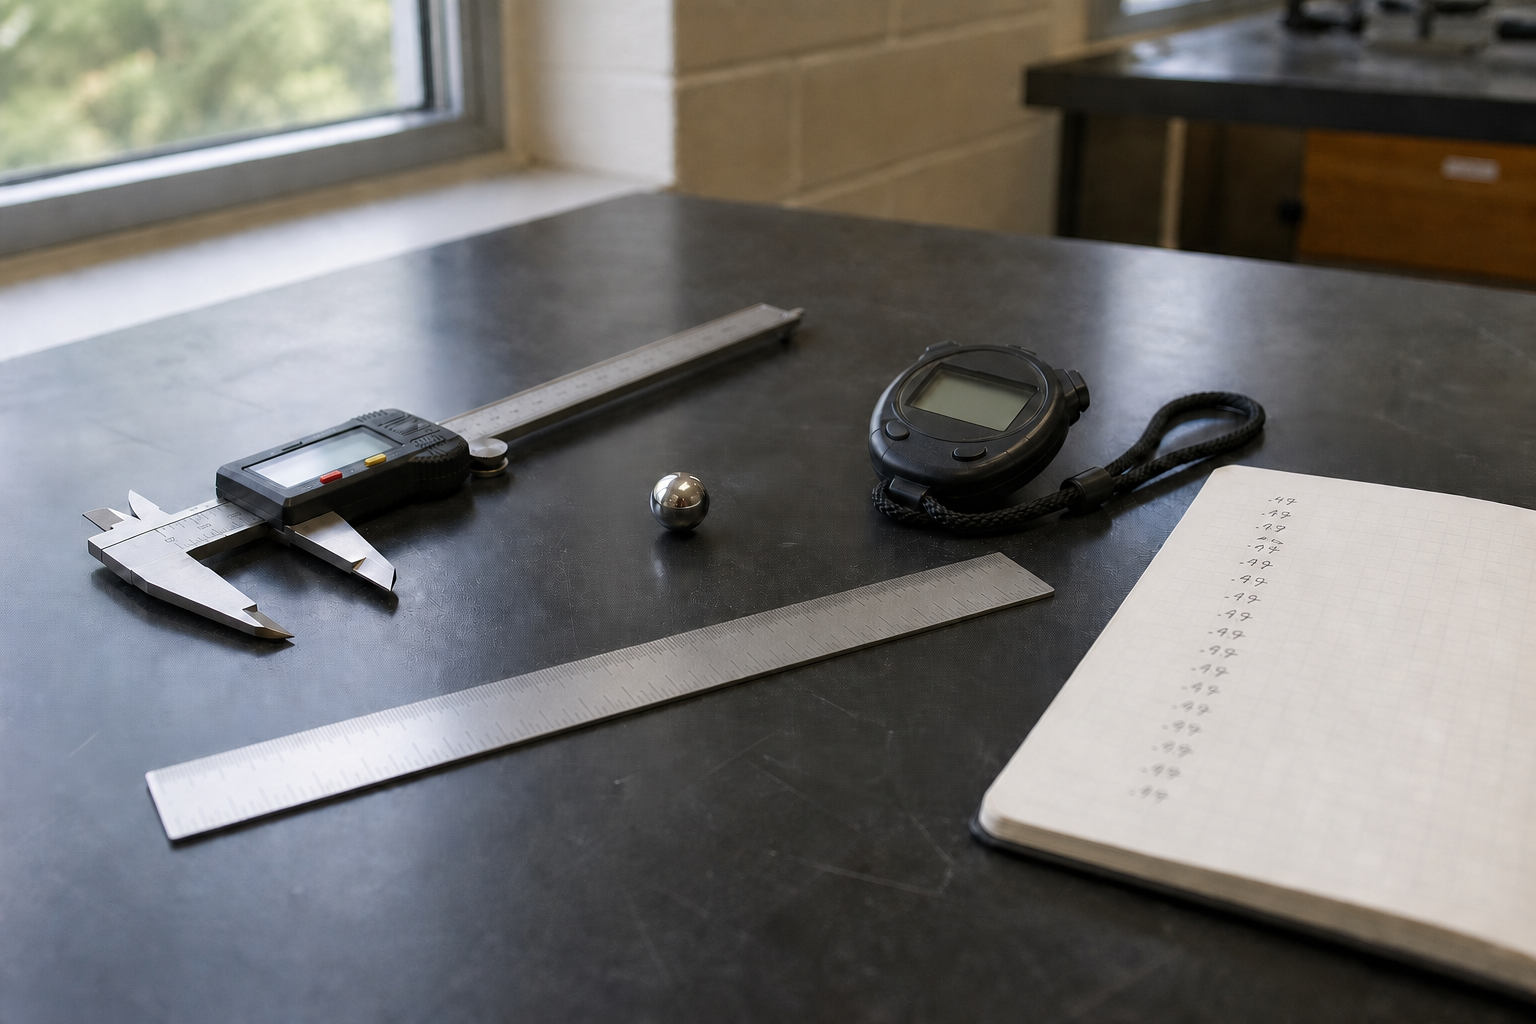
\includegraphics[width=0.60\linewidth]{images/book3/ai/b3-01-lab-bench-measuring.png}

{\small De grondstof van dit hoofdstuk: een schuifmaat, een stopwatch, een bal, een liniaal en een kolom herhaalde aflezingen die het nooit helemaal eens zijn.}
\end{omfigure}

\section{Probleem: $g$ meten met een slinger}

\begin{problem}[{Weekendopgave --- een draad, een bol, een stopwatch en een
meetlint: hoe goed kan een keukentafel het zwaartekrachtveld van de aarde
meten, en welk van haar vier getallen is de zwakke schakel}]
\label{pb:b1:units-dimensions:1}
Een slinger is een stalen bol die met een lichte draad aan een vast punt hangt;
kleine uitwijkingen hebben periode $\tau = 2\pi\sqrt{\ell/g}$, waarin $\ell$ de
afstand is van het ophangpunt tot het middelpunt van de bol. Het doel is een
waarde van $g$ met een verdedigbare onzekerheid.

\medskip
\noindent\textbf{Deel I --- Het model.}
\begin{enumerate}
  \item Controleer de homogeniteit van $\tau = 2\pi\sqrt{\ell/g}$.
  \item De bol heeft massa $m$. Beargumenteer met \omterm{def:b1:units-dimensions:dimension}{dimensies} alleen dat de
        periode niet van $m$ kan afhangen als zij alleen van $\ell$, $g$
        en $m$ afhangt.
  \item De periode hangt ook, een beetje, af van de uitwijking $\theta_0$
        van de zwaai. Waarom laat dimensieanalyse dit toe, en wat moet men
        proefondervindelijk doen om de formule bruikbaar te maken?
  \item Druk $g$ uit als functie van $\ell$ en $\tau$.
\end{enumerate}

\medskip
\noindent\textbf{Deel II --- De lengte meten.}
Het meetlint is in millimeters verdeeld; de draad is
\qty{99.0}{cm} lang van het ophangpunt tot de bovenkant van de bol, de
diameter van de bol is \qty{2.00}{cm}, beide één keer afgelezen.
\begin{enumerate}[resume]
  \item Bereken $\ell$.
  \item Bepaal de onzekerheid van type B van één aflezing op het
        meetlint.
  \item Het ophangpunt en het middelpunt van de bol lokaliseren voegt naar
        schatting $\pm\qty{5}{mm}$ mogelijke fout toe (uniform). Combineer
        die met het vorige punt tot $u(\ell)$, en geef de relatieve
        onzekerheid $u(\ell)/\ell$.
\end{enumerate}

\medskip
\noindent\textbf{Deel III --- De periode meten.}
Om de invloed van de reactietijd te beperken klokt men tien perioden. Acht
zulke metingen, in seconden: $20.12$, $20.05$, $20.18$, $20.09$, $20.15$,
$20.02$, $20.11$, $20.08$.
\begin{enumerate}[resume]
  \item Waarom tien perioden klokken in plaats van één? Waarom de meting
        acht keer herhalen?
  \item Bereken het gemiddelde $\overline{t_{10}}$ en de experimentele
        standaardafwijking $s$ van de acht metingen.
  \item Leid de \omterm{def:b1:units-dimensions:uncertainty}{standaardonzekerheid} van het gemiddelde af, dan de periode
        $\tau$ en haar onzekerheid $u(\tau)$.
  \item Vergelijk $u(\tau)/\tau$ met $u(\ell)/\ell$.
\end{enumerate}

\medskip
\noindent\textbf{Deel IV --- Het resultaat en zijn zwakke plek.}
\begin{enumerate}[resume]
  \item Bereken $g$.
  \item Schrijf $u(g)/g$ in termen van $u(\ell)/\ell$ en $u(\tau)/\tau$,
        en bereken het.
  \item Schrijf het resultaat in de standaardvorm op.
  \item Vergelijk met de referentiewaarde $\qty{9.81}{m/s^2}$ via de
        \omterm{def:b1:units-dimensions:zscore}{genormaliseerde afwijking}. Oordeel?
  \item Welke van de twee gemeten grootheden begrenst de precisie van
        $g$? Stel twee concrete verbeteringen voor en zeg met hoeveel elk
        de relatieve onzekerheid zou verkleinen.
  \item Stel dat door een slordige uitlijning elke lengte met \qty{5}{mm}
        is overschat. Zit dat in de onzekerheidsbegroting? Welke naam
        draagt dit soort fout, en hoe zou men haar opsporen?
\end{enumerate}

\medskip
\noindent\textbf{Deel V --- Vijf lengtes en een rechte.}
De proef wordt herhaald voor $\ell = 0.400$, $0.600$, $0.800$,
$1.000$ en \qty{1.200}{m}, wat $\tau^2 = 1.62$, $2.41$, $3.25$,
$4.04$ en \qty{4.84}{s^2} oplevert, elk met $u(\tau^2) \approx 1\%$.
\begin{enumerate}[resume]
  \item Waarom $\tau^2$ tegen $\ell$ uitzetten in plaats van $\tau$ tegen
        $\ell$?
  \item Bereken $\bar\ell$ en $\overline{\tau^2}$.
  \item Bereken de kleinstekwadratenrichtingscoëfficiënt $a$ en het snijpunt $b$.
  \item Leid $g$ af uit de richtingscoëfficiënt.
  \item Duid het snijpunt: wat zou een duidelijk van nul verschillende $b$
        verraden?
  \item De aanpassing op de computer geeft $u(a) = \qty{0.05}{s^2/m}$. Leid
        $u(g)$ af en schrijf het resultaat op.
  \item Vergelijk het resultaat uit Deel IV, met één lengte, met dit
        resultaat via de \omterm{def:b1:units-dimensions:zscore}{genormaliseerde afwijking}.
  \item Een student stelt voor in plaats daarvan één zwaai van een slinger
        van \qty{10}{m} in een trappenhuis te klokken, met hetzelfde
        meetlint en dezelfde stopwatch. Schat de relatieve onzekerheid op
        $g$ die dat zou opleveren, en trek een conclusie over de beste
        aanpak.
\end{enumerate}
\end{problem}
